\chapter{Design}
This section details the overall design of the Confuzzer system. We've split the
design into two major parts, the Taint System design and the Concolic System
design, as well as an additional section that covers the design of the smaller
components of the Confuzzer system.

\section{Taint System Design}
One of the major parts of this system is the system that keeps track of the
spread of Taint through a program from the tainted input that we are
testing. While many Taint Analysis systems of various sorts exist, most have to
do with doing analysis in the Intermediate Representation of a program that is
represented as part of the compilation process. Due to the lack of source code
for most programs, we have to design the system to do Taint Analysis on the
final running assembly. This presents a lot of complications since x86 assembly
doesn't provide nice semantics for figuring out what registers are tainted by an
operation or categories to separate the various assembly instructions.

\begin{figure}[htbp]
 \centering
 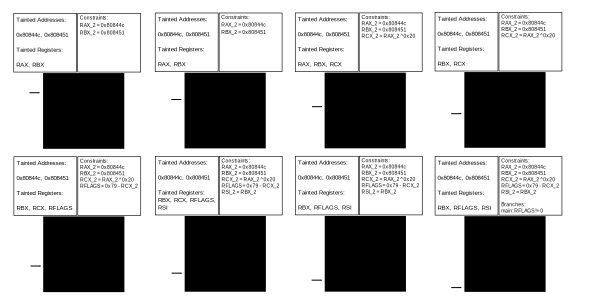
\includegraphics{taintprop}
 \caption{Taint Propogation Example}
 \label{figure:taintprop}
\end{figure}

The basic design of the taint system is that we initially capture any reads from
the file descriptor referencing our ``tainted input''. We can then keep track of
any memory addresses or locations that this ``tainted input'' is stored
in. We also mark each of the original reads from the tainted file with a special
marker that is then used by the Concolic System. Then, we analyze each
instruction in the program and if its a read from a tainted location (memory or
register), we create a new constraint representing the instruction and taint the
resulting location. In this way, as the program executes the set of tainted
registers and addresses slowly changes at each instruction. Finally, we can keep
track of any branches that occur in the program and check whether they are
controlled by the ``tainted input'' by seeing if the values the branch is
depended on is tainted at that time. Figure \ref{figure:taintprop} shows an
example of how this system works.

\begin{figure}[ht]
 \centering
 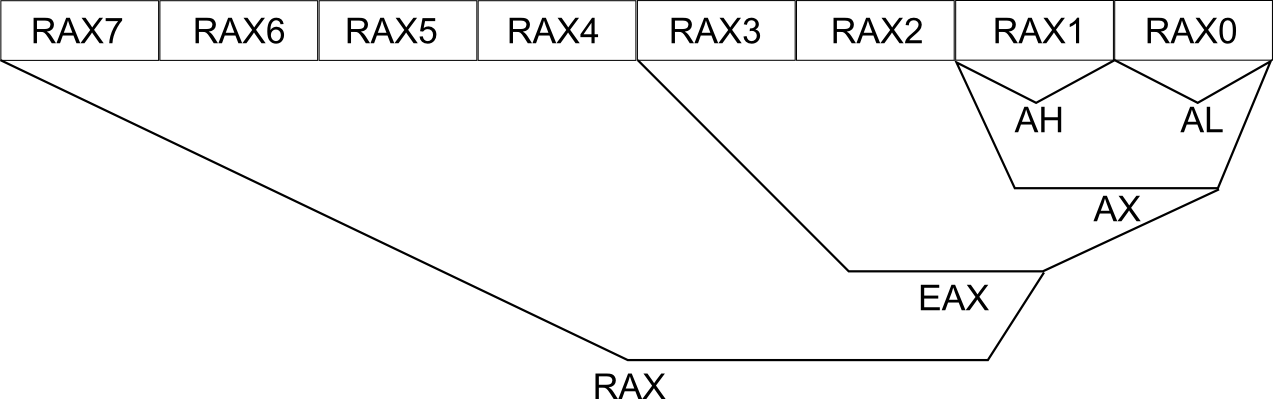
\includegraphics{taintregs}
 \caption{Register Chunks Example}
 \label{figure:taintregs}
\end{figure}

However this design doesn't deal with the fact that we have instructions that
move registers of differing lengths. In order to deal with this, we instead keep
track of each register as chunks of 8 bits. Therefore most registers, which tend
to be 64-bit, are made of 8 chunks numbered $R{\it N}X0$ through $R{\it  N}X7$.  
Depending on the size of the operation that moves data around, we copy
over a certain series of register chunks over, keeping the previous values for
the uncopied registers. Figure \ref{figure:taintregs} shows the layout described
and how the various register chunks are related.

Each tainted operation we encounter then generates the constraints depicted in
Figure \ref{figure:regexample}, which while more than the original design
doesn't add that much complexity for z3 to solve against, since most of the
constraints are under constrained or simple substitutions.

\begin{figure}[t]
\centering
\begin{verbatim}
Tainted: RAX0_1, RAX1_1
Instruction: xor ax, 0x2020
Tainted: RAX0_1, RAX1_1, RAX0_2, RAX1_2

New Constraints:
 RAX_AX_1 = {RAX1_1, RAX0_1}
 RAX_AX_2 = OP(RAX_AX_1 + 0x2020)
 RAX1_2 = RAX_AX_2[1]
 RAX0_2 = RAX_AX_2[0]
\end{verbatim}
\caption{Register Constraints Example}
\label{figure:regexample}
\end{figure}

Once the Taint Analysis system has finished generating the list of tainted
instructions and a semantic for how the registers are altered, it produces a
text file listing all the tainted branches that were encountered, along with the
list of tainted instructions/constraints. While the instructions are separated
into separate registers and rough constraints at the taint analysis stage, it
isn't until the generated file enters the Concolic system that the constraints
are parsed and turned into a form more suitable for our constraint solver.

\section{Concolic System Design}
The Concolic System has many components working together to generate new inputs
and to call out to the Taint Analysis system. It first generates an initial
blank input which is sent to the Taint Analysis system. Then, for each input it
has sent off it first parses the response, generating SMT constraints
representing the state of the program and each branching point. Then it proceeds
to attempt to solve the constraints for new inputs that can once again be sent
off to the Taint Analysis system. If we have already observed an input, we skip
it since we've already parsed it, and once we are unable to generate new inputs
that traverse unexplored parts of the program, we conclude the fuzzing. We'll
discuss each of these stages in turn.

\subsection{Taint Analysis Parsing}
This stage turns the Taint Analysis output from something like 
``RFLAGS\_0\_1: cmp al, 0x6c ::: RFLAGS\_0\_1 = OP(RAX\_0\_1, 0x6c)'' into a SMT
equation of the form ``RFLAGS\_0\_1 == 0x6C - RAX\_0\_1''. We don't generate the
actual SMT form until this stage in order to allow the Taint Analysis system to
be disconnected from the format of the SMT system we are using. This stage is
actually split into two parts, one to handle the parsing of the actual branches
that have been encountered and another to parse the general
instructions/constraints that we've picked up throughout the execution of the
program.

For each branch, we also need to figure out whether the branch was taken during
this execution so that the Path Exploration system can determine what branches
haven't been visited. Since almost all branches are based on the state of
RFLAGS, we also have the Taint Analysis provide the concrete values of RFLAGS so
that we can determine whether the path has been taken depending on the opcode of
the branch instruction.

For general instructions/constraints, we parse each instruction to convert the
opcode into an actual operation between the arguments of the instruction. There
are three categories of instructions, those that take a single argument, those
that take two arguments, and finally those that also modify RFLAGS. Using both
the semantics of the arguments and the opcode, we can determine the appropriate
operation to perform between the operations.

Once we've gathered a series of SMT equations representing all the steps of the
program execution, as well as a separate series of equations representing each
of the branches we've taken, we pass this onto the Path Exploration system to
generate subsets of the branch equations for Input Generation.

\subsection{Path Exploration}
Once we've generated the initial SMT equations, we need to start generating the
various different sets of branch paths we want to explore in subsequent
tests. The way we generate each of these new branch paths is by going through
each of the branches we've hit, and keeping all previous branch constraints
while we negate the current branch constraint. Figure \ref{figure:pathexplore}
shows the initial path that we've explored, as well as the additional paths
we'll try exploring in the new inputs. We don't worry about de-duplicating paths
at this point since we'll de-duplicate repeated inputs as part of the input
generation phase.

\begin{figure}[ht]
 \centering
 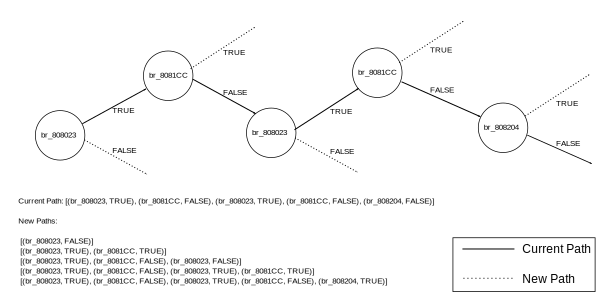
\includegraphics{pathexplore}
 \caption{Path Exploration Example}
 \label{figure:pathexplore}
\end{figure}

Once we've figured out which branch constraints to keep and which to negate, we
can simply add a new constraint of ``AND(branches[:i], NOT(branches[i]))''. Once
we have all the constraints, we send them to the SMT solver to solve and
generate concrete values for all the variables. Once this step is done, the
result can be passed to the Input Generation phase to create new test cases.

\subsection{Input Generation}


\section{Minor Component Design}
